\documentclass{mpaper}

\usepackage{graphicx}
\usepackage{multirow}
\usepackage{booktabs}
\usepackage[format=plain, labelfont={bf},textfont=it,tableposition=above]{caption}

\begin{document}

\title{mmFace: 3D Face Recognition with RGB and Millimetre Wave Radar}
\author{Stergious Aji}
\matricnum{2546916A}

\maketitle

\begin{abstract}
    TODO
    % According to Simon Peyton Jones, an abstract should address four key questions. First, what is the problem that this paper tackles? Second, why is this an interesting problem? Third, what is the solution this paper proposes? Finally, why is the proposed solution a good one?


\end{abstract}

% This paper outlines the standard template for a final MSci project report submission at the School of Computing Science in the University of Glasgow. In earlier years, MSci students at the School of Computing Science\footnote{\url{https://www.gla.ac.uk/computing}}, University of Glasgow, were expected to produce a full-length dissertation. Now, the requirement is for MSci students to write a paper of up to 14 pages in length, using the supplied \texttt{mpaper} \LaTeX style file.

% The precise structure of an MSci paper is not mandated, but it should probably cover in detail the following aspects of the project.
% \begin{enumerate}
% \item General description of the problem, motivation, relevance
% \item Background information, possibly including a literature survey
% \item Description of approach taken to solve the problem, including high-level design and lower-level implementation details as appropriate
% \item Evaluation, qualitative or quantitative as appropriate
% \item Conclusion, including scope for future work
% \end{enumerate}

\section{Introduction}
Facial recognition technology is a key area of research within the field of computer vision, with widespread applications across areas such as security surveillance, forensic analysis, and human-computer interaction. Its most prominent use case lies in biometric authentication, allowing individuals access to their personal devices or restricted areas. This enables a non-invasive, hands-free approach to identity verification, removing the need to recall passwords. Furthermore, facial biometrics are naturally more accessible than other forms such as fingerprints, iris, or palm prints \cite{zhou20183d}.

Since its inception in the 1960s, facial recognition systems have evolved drastically. The pioneering work by Bledsoe \cite{bledsoe1966model} first distinguished faces by comparing distances of manually annotated landmark features such as the nose, eyes, and mouth. In more recent years, the advent of deep learning has enhanced the performance and efficiency of human face classification, benefitting from the vast online repositories of face images.  Nevertheless, these systems primarily rely on images captured by RGB cameras, making them susceptible to variations in lighting and pose \cite{xu2004depth}. By incorporating depth data, which draws attention to the geometric details of the face, the effect of such environmental factors can be mitigated. Moreover, the transition to three-dimensional face recognition not only improves accuracy, but also enhances the security of biometric systems against spoofing attacks \cite{wen2015face}.



\subsection{Motivation}
The popularity of 3D face recognition is on the rise, evidenced by its adoption in smartphones with the likes of Apple and their Face ID \cite{apple-faceid} technology. This growing demand has pushed the commercialisation of depth-sensing technology to smaller form factors, enabling it to operate efficiently in real-time on mobile devices \cite{soumya2023recent}. Face ID, in particular, has achieved a level of security that allows its integration into services like Apple Pay. However, the use of costly proprietary hardware and restrictive patents by Apple make it harder for smaller companies to adopt an equally compact and secure face recognition system.

Depth cameras used in this context typically employ an active face acquisition method. This is where non-visible light is projected onto the face and reflected back, allowing sensors to measure and map facial features. The most common approach involves lidar cameras, emitting waves in the near-infrared spectrum, due to their ability to capture a dense 3D map of the subject's face \cite{wang2020evolution}. However, its weakness in penetrating materials such as clothing and hair is a notable limitation. In contrast, millimetre radar waves (mmWaves) can penetrate such materials to directly reach the dermal layer of the skin \cite{vizard2006advances}, potentially offering better performance in scenarios involving facial hair, or even within challenging environmental conditions such as rain or fog.

Research into the efficacy of radar waves for 3D face recognition is relatively sparse, but recent studies show positive results \cite{hof2020face, lim2020dnn,kim2020face, pho2021radar,challa2021face}. Radar sensors are generally more cost-effective, both in terms of acquisition and computation, as they consume less power compared to NIR-based sensors. However, it is important to note the trade-off, as mmWaves tend to yield a sparser representation meaning a lower accuracy in comparison. This could impact recognition performance where precision in detecting and mapping facial features is paramount. This project aims to therefore explore counter-balancing this limitation with the information gained from colour images, potentially paving the way for more resilient and versatile systems. 


\subsection{Research Aims}
This project aims to explore the effectiveness of using RGB cameras in conjunction with mmWave radar sensors for 3D facial recognition. Since there are no appropriate datasets available for this purpose, we collate this data ourselves. We use the Intel RealSense L515 RGB-D camera \cite{intel-l515} for photographing an individual's face. Meanwhile, the Google Soli 60 GHz radar sensor \cite{lien2016soli} will be employed to gather depth information by transmitting and measuring millimetre waves reflected from the target.

We initially planned to gather face data from approximately 50 participants, however, only 21 participants came forward within the limited timeframe. We aim to obtain face data under various conditions including diverse poses, lighting environments, and common occlusion scenarios. The objective is to empirically validate the benefits of utilising mmWave technology in this context. We hypothesise that this approach would yield a system that is invariant to pose, lighting, and occlusion compared to using RGB or depth information alone.

Next, we plan to develop a novel face recognition model using a deep Convolutional Neural Network. This model will be trained on the captured data in order to learn facial features from both the RGB and depth characteristics acquired from the Soli sensor. We also intend to investigate different techniques in fusing these two modalities, aiming to pinpoint the most effective strategy that provides rich and distinctive representations, for accurate face classification performance. The model's effectiveness will be benchmarked against prior radar-based facial recognition systems, as well as, a comparison to solely using RGB data.

The main research aims for this project are summarised and listed below:

\begin{enumerate}
    \item Explore the feasibility of using RGB cameras in conjunction with mmWave radar sensors for 3D facial recognition.
    \item Collate a face dataset of colour images and mmWave signatures from a diverse array of 50 participants. The Intel Realsense L515 \cite{intel-l515} and the Google Soli chip \cite{lien2016soli} will be employed to accomplish this. This data will be obtained under various conditions including diverse poses, lighting environments and common occlusion scenarios.
    \item Empirically test the hypothesis that incorporating the depth information from the mmWave face signatures yields a more robust system, invariant to pose, lighting, occlusion, and spoofing.
    \item Develop a novel face recognition model that can be trained on both modalities simultaneously. This model should be able to classify a given face as well as identify if it is live or fake.
    \item Investigate various feature fusion methods to determine the optimal approach for integrating the RGB and mmWave facial features. This aims to yield richer, more distinctive representations for better face classification performance.
    \item Investigate the proposed model's effectiveness at classifying unseen faces and identifying their liveness compared to solely using RGB data.
\end{enumerate}


\section{Background}

\subsection{Related Work}
The use of millimetre waves for face identification is a relatively new research field, spurred by the commercialisation of radar sensor technology. One of the earliest studies found to investigate human identification using mmWaves can be traced back to 2019, conducted by Zhao et al. \cite{zhao2019mid}. Although this paper focuses on classifying subjects by their gait and body shape rather than facial features, it demonstrates the ability of mmWaves to encapsulate the subtle idiosyncrasies among individuals. These nuanced differences are vital for learning models to effectively differentiate between unique subjects, leading to high classification accuracies.

Following this, Hof et al. \cite{hof2020face} proposed a Deep Neural Network (DNN) based Autoencoder that can distinguish human faces captured by an 802.11ad/y networking chipset operating at a centre frequency of 60 GHz. The Autoencoder is able to encode mmWave face signatures of over 200 individuals with enough separation to distinguish between positive and negative instances by measuring their Mean Squared Error (MSE) against reference facial embeddings. The study conducted an extensive data collection process, capturing face scans of 206 participants comprising various genders and ages, in five different poses: frontal, as well as, $15^\circ$ and $25^\circ$ head rotations to the left and right. This collection was subsequently made available through an IEEE Data Port \cite{mmwavefacedata}. While this dataset encapsulates faces from a wide range of people, including some with beards and spectacles, it lacks representation of other common occlusion scenarios like head accessories, that our project aims to explore. Moreover, the study utilised a larger sensor containing a total of 1024 transmit and receiver antenna pairs, found to capture redundant information. This is in contrast to the compact Soli chip with a single transmit and three receiver antennas, intended to work within a smartphone. The study simulated the effect of reducing the antenna count to 10, markedly decreasing the distinctiveness of facial signatures. Promisingly, increasing the number of neurons in their Neural Network and an additional hidden layer could compensate for this reduction, maintaining high accuracy.

Lim et al. \cite{lim2020dnn} proposes another Deep Neural Network model, however with a more traditional Multi-Layer Perceptron (MLP) architecture where every layer is fully connected to adjacent ones. The study utilised a small-scale, 61 GHz FMCW radar sensor developed by bitsensing Inc. \cite{bitsensing2020bts60}, comparable to the Google Soli with a single transmit and three receiver antennas. The model attained a mean classification accuracy of 92\% across eight subjects, surpassing the performance of both, a Support Vector Machine (SVM), and a tree-based Ensemble Learning approach trained on the same face signatures. It is important to note the relatively small-sized dataset used to train the model, raising concerns about potential overfitting as the data is not representative enough. The paper provides limited details on the data collection methodology used, only mentioning that the facial distances ranged from 30 cm to 50 cm. It can be assumed then that the study likely focussed on frontal poses without any occlusions for all eight subjects. The research also explored the impact of using a single receiving antenna, which resulted in a reduced accuracy of 73.7\%. This finding is in line with Hof et al.'s \cite{hof2020face} observation that an increased number of receiving antennas can enhance classification accuracy by the ability to capture more nuanced facial features. The paper also suggests that a CNN may be more appropriate if signals were stacked on the time axis rather than the frequency axis.

During the same period, Kim et al. \cite{kim2020face} conducted research using an identical 61 GHz FMCW radar sensor from bitsensing Inc., featuring a range resolution of 2.5 cm. Their study introduces a CNN model comprising three convolutional layers and three fully connected layers. The radar data underwent heavy preprocessing to transform it into a more image-like format suitable for the CNN model. With a data split of 70\%/15\%/15\% for training, validation, and testing, the model achieved an average classification accuracy of 98.7\% on a limited dataset of only three individuals. Interestingly, the study also examined the impact of wearing cotton masks. The results showed a minimal drop in average classification accuracy by 0.9\%, which is encouraging for the objectives of our project. However, these findings are to be taken with caution due to the small size of the dataset. It remains unclear whether this level of performance would hold consistently across a larger and more diverse group of subjects, with more varied occlusions.

Pho et al. \cite{pho2021radar} adopts a One-Shot Learning approach to the problem. This is where the model is trained with a single or only a few labelled instances, beneficial when there is a lack of training samples available. The proposed method constitutes a Siamese structure of two identical CNNs with shared parameters that map the input radar signals into a latent space. A distance metric between the outputs of both CNNs is used during the training and testing phases to measure the similarity between face inputs. The model is specifically trained for \textit{binary classification} by inputting pairs of face signatures from either the same or different people. This process resulted in the model learning embeddings that push different faces into distinct Euclidean regions of the embedding space. The same bitsensing Inc. BTS60 chipset, used by Lim et al. and Kim et al. \cite{lim2020dnn, kim2020face}, is employed to capture 500 frames of the faces of eight participants. An average classification of 97.6\% was achieved, an improvement over the previous DNN model by Lim et al. involving the same number of people. t-Stochastic Neighbour Embedding (t-SNE) \cite{van2008visualizing} is then applied for dimensionality reduction. The resulting visualisations demonstrated that the one-shot Siamese network effectively separated each individual's face into exclusive regions, simplifying the classification task. Although a small dataset is used,\,only encompassing frontal poses with no occlusion\,settings, the proposed method is well documented and is likely robust against larger datasets.

Challa et al. \cite{challa2021face} employs two different machine learning models on the dataset made available through the IEEE port \cite{mmwavefacedata}. Their approach began with CNN-based Autoencoders followed by a Random Forest Ensemble Learning approach. A total of nine Autoencoders were built, each tailored to different frame rates, focusing on compressing and learning to reconstruct the original data from its compressed, latent form. The Autoencoders were trained using randomly selected data samples from a subset of 186 mmWave face signatures. The flattened and labelled outputs were then used to train and test nine discrete Random Forest models using identical hyperparameters, as recommended by the Sci-kit library. This methodology yielded impressive results, achieving an average classification accuracy of 99.98\% using all 1400 frames per individual. Even reducing the number of frames to 70 per person, the model was able to maintain a high accuracy of 97.1\%. The paper presents an approach that is unique in comparison to the rest of the research papers tackling this subject, showcasing an efficient model that is able to be deployed on mobile chips.

The research in this area exclusively focuses on utilising data from radar sensors, largely driven by concerns of privacy preservation. However, a significant limitation of this approach is the required duration for capturing an accurate facial scan. The sensor needs to operate for several seconds, typically in the range between 10 and 15 seconds, in order to obtain a detailed scan. Such a time frame is impractical in real-world situations, as it necessitates the subject to remain motionless for a prolonged period. Up to this point, no study was found to explore the potential benefits of combining radar signatures with corresponding RGB data to enhance facial recognition capabilities. Given the high performance of existing deep learning models using RGB images alone, such as InsightFace \cite{deng2018arcface}, integrating these models with mmWave radar data presents a promising avenue. This combination could accelerate face acquisition time, while leveraging the advantages of mmWaves in terms of their robustness to lighting variations and occlusions.



\section{Methodology}

\subsection{Data Acquisition}

\begin{figure}[h!]
    \centering
    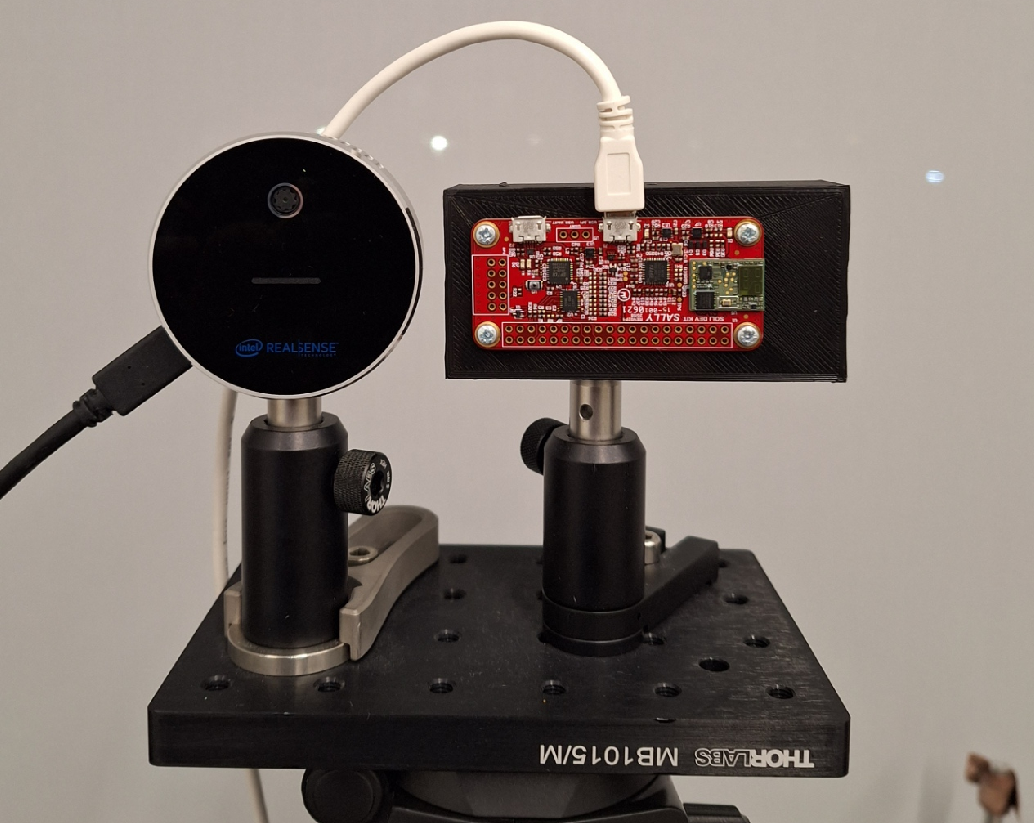
\includegraphics[width=0.35\textwidth]{diagrams/equipment.pdf}
    \vspace{0.2cm}
    \caption{Equipment: Intel Realsense L515 RGB-D Camera (Left) and the Google's Soli 60 GHz radar sensor (right)}
    \label{fig:equipment}
\end{figure}

\begin{figure}[h!]
    \centering
    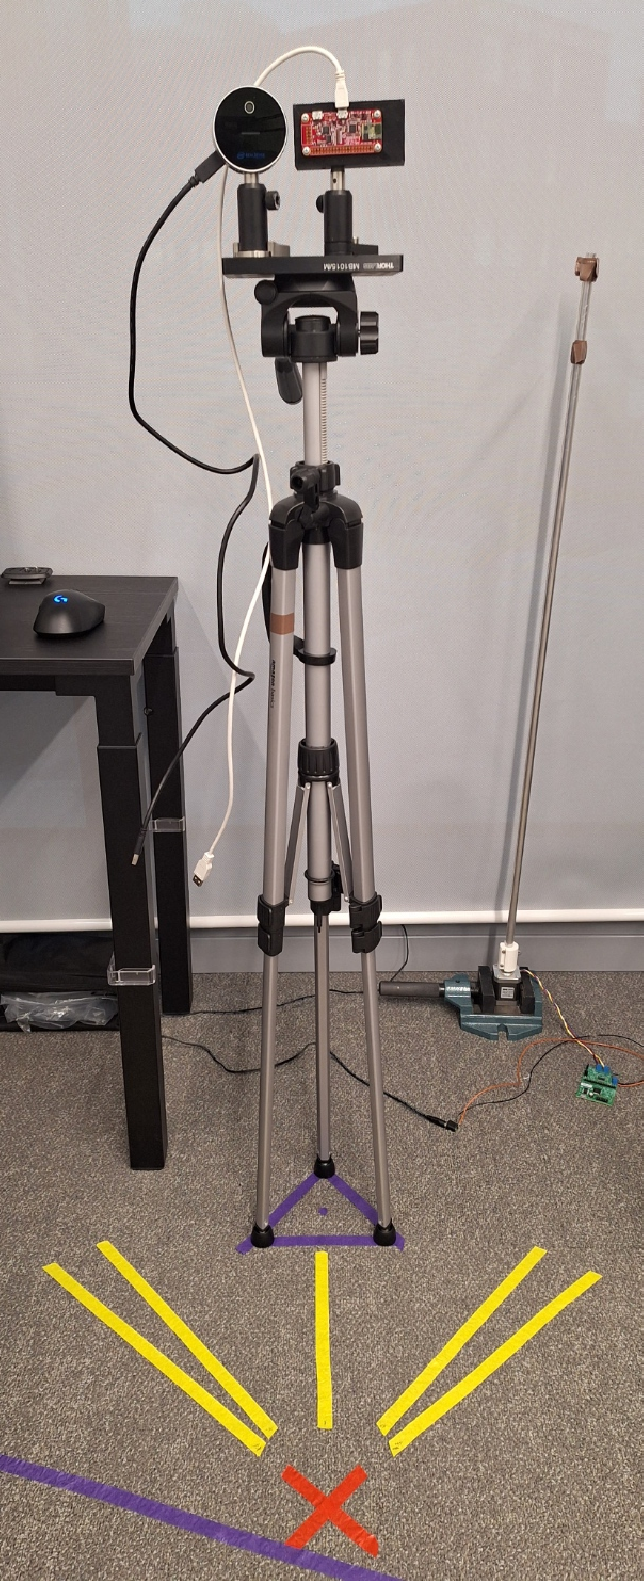
\includegraphics[width=0.3\textwidth, height=12.5cm]{diagrams/experiment_setup.pdf}
    \caption{Experiment Setup}
    \label{fig:experiment_setup}
\end{figure}


\subsection{mmFace}

\begin{figure*}[h!]
    \centering
    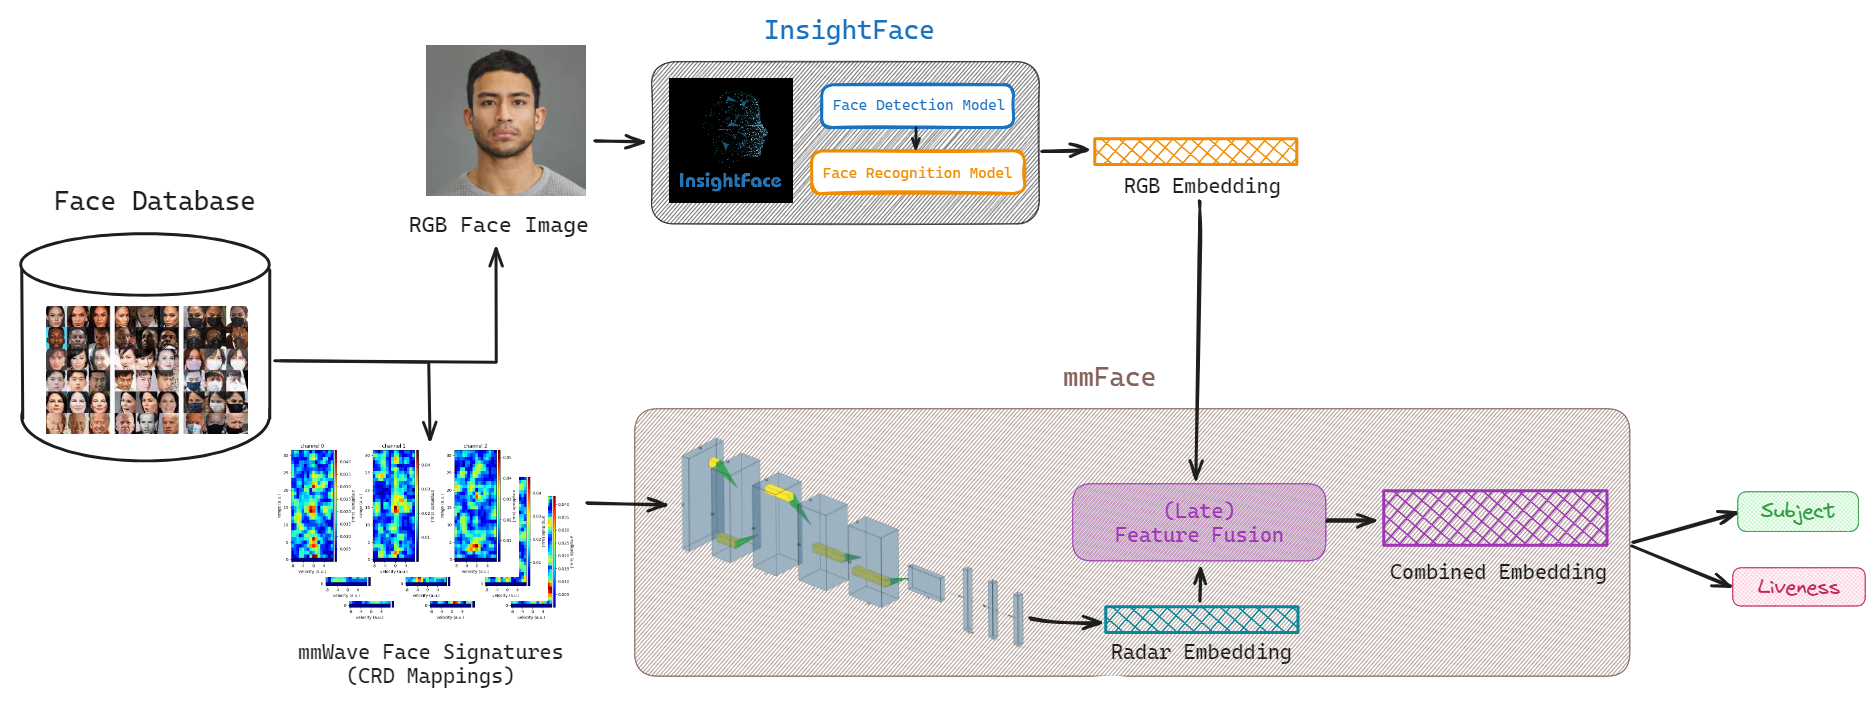
\includegraphics[width=1\textwidth]{diagrams/model_workflow.png}
    \caption{Workflow Diagram}
    \label{fig:model_workflow}
\end{figure*}

\begin{figure*}[h!]
    \centering
    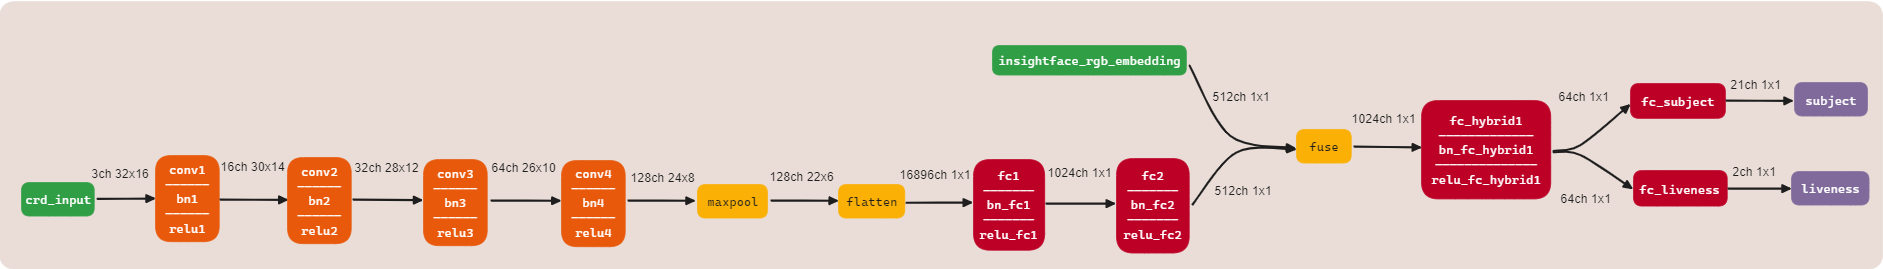
\includegraphics[width=1\textwidth]{diagrams/model_architecture.png}
    \caption{Architecture Diagram}
    \label{fig:model_architecture}
\end{figure*}


\section{Evaluation}

\subsection{Results}
% TODO: TABLE
% \begin{table}[htbp]
%     \centering
    
%     \begin{tabular}{lcccc}
%       \toprule
%       \multirow{2}{*}{\textbf{Feature Fusion}} & \multicolumn{2}{c}{\textbf{Subject}} & \multicolumn{2}{c}{\textbf{Liveness}} \\
%       \cmidrule(lr){2-3} \cmidrule(lr){4-5}
%        & \textbf{Accuracy} & \textbf{F1 Score} & \textbf{Accuracy} & \textbf{F1 Score} \\
%       \midrule
%       Concatenate & 83.70\% & 0.8347 & 99.60\% & 0.9932 \\
%       Add & 62.97\% & 0.6291 & 99.20\% & 0.9911 \\
%       Multiply & 87.10\% & 0.8543 & 96.66\% & 0.9481 \\
%       Pairwise Dot Average & 88.83\% & 0.8464 & 80.81\% & 0.7699 \\
%       Pairwise Dot Max & 82.70\% & 0.7905 & 72.84\% & 0.6962 \\
%       Pairwise Dot Flatten & 86.66\% & 0.8480 & 94.74\% & 0.9270 \\
%       Multi-Head Attention & 86.28\% & 0.7984 & 96.41\% & 0.8922 \\
%       \bottomrule
%     \end{tabular}
%     \caption{Results of Feature Fusion Techniques}
%     \label{tab:results}
%   \end{table}

%   \begin{table}[htbp]
%     \centering
%     \begin{tabular}{lcc}
%         \toprule
%         \textbf{Feature Fusion}   & \textbf{Macro-Averaged AUC} & \textbf{KL Divergence} \\
%         \midrule
%         Concatenate          & 0.7427                      & 0.9501                 \\
%         Add                  & 0.6672                      & 1.2934                 \\
%         Multiply             & 0.7282                      & 0.5468                 \\
%         Pairwise Dot Average & 0.9204                      & 0.2155                 \\
%         Pairwise Dot Max     & 0.8511                      & 0.2394                 \\
%         Pairwise Dot Flatten & 0.8562                      & 0.3653                 \\
%         Multi-Head Attention & 0.8229                      & 0.4775                 \\
%         \bottomrule
%     \end{tabular}
%     \caption{Performance Metrics for Feature Fusion Techniques}
%     \label{tab:metrics}
% \end{table}



\section{Conclusions}



\subsection{Future Work}


{\bf Acknowledgments.}
This is optional; it is a location for you to thank people, most probably your family and your supervisor.


\bibliographystyle{unsrt}
\bibliography{l5proj}

\end{document}
